% Options for packages loaded elsewhere
\PassOptionsToPackage{unicode}{hyperref}
\PassOptionsToPackage{hyphens}{url}
%
\documentclass[
  english,
  man]{apa6}
\usepackage{amsmath,amssymb}
\usepackage{lmodern}
\usepackage{ifxetex,ifluatex}
\ifnum 0\ifxetex 1\fi\ifluatex 1\fi=0 % if pdftex
  \usepackage[T1]{fontenc}
  \usepackage[utf8]{inputenc}
  \usepackage{textcomp} % provide euro and other symbols
\else % if luatex or xetex
  \usepackage{unicode-math}
  \defaultfontfeatures{Scale=MatchLowercase}
  \defaultfontfeatures[\rmfamily]{Ligatures=TeX,Scale=1}
\fi
% Use upquote if available, for straight quotes in verbatim environments
\IfFileExists{upquote.sty}{\usepackage{upquote}}{}
\IfFileExists{microtype.sty}{% use microtype if available
  \usepackage[]{microtype}
  \UseMicrotypeSet[protrusion]{basicmath} % disable protrusion for tt fonts
}{}
\makeatletter
\@ifundefined{KOMAClassName}{% if non-KOMA class
  \IfFileExists{parskip.sty}{%
    \usepackage{parskip}
  }{% else
    \setlength{\parindent}{0pt}
    \setlength{\parskip}{6pt plus 2pt minus 1pt}}
}{% if KOMA class
  \KOMAoptions{parskip=half}}
\makeatother
\usepackage{xcolor}
\IfFileExists{xurl.sty}{\usepackage{xurl}}{} % add URL line breaks if available
\IfFileExists{bookmark.sty}{\usepackage{bookmark}}{\usepackage{hyperref}}
\hypersetup{
  pdftitle={Demanding resources: Agreement of perceptions for challenge and resource characteristics},
  pdfauthor={John Kulas1 \& Alicia Stachowski2},
  pdflang={en-EN},
  pdfkeywords={keywords},
  hidelinks,
  pdfcreator={LaTeX via pandoc}}
\urlstyle{same} % disable monospaced font for URLs
\usepackage{graphicx}
\makeatletter
\def\maxwidth{\ifdim\Gin@nat@width>\linewidth\linewidth\else\Gin@nat@width\fi}
\def\maxheight{\ifdim\Gin@nat@height>\textheight\textheight\else\Gin@nat@height\fi}
\makeatother
% Scale images if necessary, so that they will not overflow the page
% margins by default, and it is still possible to overwrite the defaults
% using explicit options in \includegraphics[width, height, ...]{}
\setkeys{Gin}{width=\maxwidth,height=\maxheight,keepaspectratio}
% Set default figure placement to htbp
\makeatletter
\def\fps@figure{htbp}
\makeatother
\setlength{\emergencystretch}{3em} % prevent overfull lines
\providecommand{\tightlist}{%
  \setlength{\itemsep}{0pt}\setlength{\parskip}{0pt}}
\setcounter{secnumdepth}{-\maxdimen} % remove section numbering
% Make \paragraph and \subparagraph free-standing
\ifx\paragraph\undefined\else
  \let\oldparagraph\paragraph
  \renewcommand{\paragraph}[1]{\oldparagraph{#1}\mbox{}}
\fi
\ifx\subparagraph\undefined\else
  \let\oldsubparagraph\subparagraph
  \renewcommand{\subparagraph}[1]{\oldsubparagraph{#1}\mbox{}}
\fi
% Manuscript styling
\usepackage{upgreek}
\captionsetup{font=singlespacing,justification=justified}

% Table formatting
\usepackage{longtable}
\usepackage{lscape}
% \usepackage[counterclockwise]{rotating}   % Landscape page setup for large tables
\usepackage{multirow}		% Table styling
\usepackage{tabularx}		% Control Column width
\usepackage[flushleft]{threeparttable}	% Allows for three part tables with a specified notes section
\usepackage{threeparttablex}            % Lets threeparttable work with longtable

% Create new environments so endfloat can handle them
% \newenvironment{ltable}
%   {\begin{landscape}\begin{center}\begin{threeparttable}}
%   {\end{threeparttable}\end{center}\end{landscape}}
\newenvironment{lltable}{\begin{landscape}\begin{center}\begin{ThreePartTable}}{\end{ThreePartTable}\end{center}\end{landscape}}

% Enables adjusting longtable caption width to table width
% Solution found at http://golatex.de/longtable-mit-caption-so-breit-wie-die-tabelle-t15767.html
\makeatletter
\newcommand\LastLTentrywidth{1em}
\newlength\longtablewidth
\setlength{\longtablewidth}{1in}
\newcommand{\getlongtablewidth}{\begingroup \ifcsname LT@\roman{LT@tables}\endcsname \global\longtablewidth=0pt \renewcommand{\LT@entry}[2]{\global\advance\longtablewidth by ##2\relax\gdef\LastLTentrywidth{##2}}\@nameuse{LT@\roman{LT@tables}} \fi \endgroup}

% \setlength{\parindent}{0.5in}
% \setlength{\parskip}{0pt plus 0pt minus 0pt}

% Overwrite redefinition of paragraph and subparagraph by the default LaTeX template
% See https://github.com/crsh/papaja/issues/292
\makeatletter
\renewcommand{\paragraph}{\@startsection{paragraph}{4}{\parindent}%
  {0\baselineskip \@plus 0.2ex \@minus 0.2ex}%
  {-1em}%
  {\normalfont\normalsize\bfseries\itshape\typesectitle}}

\renewcommand{\subparagraph}[1]{\@startsection{subparagraph}{5}{1em}%
  {0\baselineskip \@plus 0.2ex \@minus 0.2ex}%
  {-\z@\relax}%
  {\normalfont\normalsize\itshape\hspace{\parindent}{#1}\textit{\addperi}}{\relax}}
\makeatother

% \usepackage{etoolbox}
\makeatletter
\patchcmd{\HyOrg@maketitle}
  {\section{\normalfont\normalsize\abstractname}}
  {\section*{\normalfont\normalsize\abstractname}}
  {}{\typeout{Failed to patch abstract.}}
\patchcmd{\HyOrg@maketitle}
  {\section{\protect\normalfont{\@title}}}
  {\section*{\protect\normalfont{\@title}}}
  {}{\typeout{Failed to patch title.}}
\makeatother
\shorttitle{Demanding Resources}
\keywords{keywords\newline\indent Word count: X}
\DeclareDelayedFloatFlavor{ThreePartTable}{table}
\DeclareDelayedFloatFlavor{lltable}{table}
\DeclareDelayedFloatFlavor*{longtable}{table}
\makeatletter
\renewcommand{\efloat@iwrite}[1]{\immediate\expandafter\protected@write\csname efloat@post#1\endcsname{}}
\makeatother
\usepackage{lineno}

\linenumbers
\usepackage{csquotes}
\ifxetex
  % Load polyglossia as late as possible: uses bidi with RTL langages (e.g. Hebrew, Arabic)
  \usepackage{polyglossia}
  \setmainlanguage[]{english}
\else
  \usepackage[main=english]{babel}
% get rid of language-specific shorthands (see #6817):
\let\LanguageShortHands\languageshorthands
\def\languageshorthands#1{}
\fi
\ifluatex
  \usepackage{selnolig}  % disable illegal ligatures
\fi
\newlength{\cslhangindent}
\setlength{\cslhangindent}{1.5em}
\newlength{\csllabelwidth}
\setlength{\csllabelwidth}{3em}
\newenvironment{CSLReferences}[2] % #1 hanging-ident, #2 entry spacing
 {% don't indent paragraphs
  \setlength{\parindent}{0pt}
  % turn on hanging indent if param 1 is 1
  \ifodd #1 \everypar{\setlength{\hangindent}{\cslhangindent}}\ignorespaces\fi
  % set entry spacing
  \ifnum #2 > 0
  \setlength{\parskip}{#2\baselineskip}
  \fi
 }%
 {}
\usepackage{calc}
\newcommand{\CSLBlock}[1]{#1\hfill\break}
\newcommand{\CSLLeftMargin}[1]{\parbox[t]{\csllabelwidth}{#1}}
\newcommand{\CSLRightInline}[1]{\parbox[t]{\linewidth - \csllabelwidth}{#1}\break}
\newcommand{\CSLIndent}[1]{\hspace{\cslhangindent}#1}

\title{Demanding resources: Agreement of perceptions for challenge and resource characteristics}
\author{John Kulas\textsuperscript{1} \& Alicia Stachowski\textsuperscript{2}}
\date{}


\authornote{

Add complete departmental affiliations for each author here. Each new line herein must be indented, like this line.

Enter author note here.

Correspondence concerning this article should be addressed to John Kulas. E-mail: \href{mailto:jtkulas@ergreports.com}{\nolinkurl{jtkulas@ergreports.com}}

}

\affiliation{\vspace{0.5cm}\textsuperscript{1} eRg\\\textsuperscript{2} University of Wisconsin - Stout}

\abstract{
568 workers rated job characteristics in terms of relevance as well as perceptions as challenges, hindrances and resources. We find strong associations between characteristics such that what is viewed as a ``resource'' is also very often considered a ``challenge.'' This agreement was moderated by the nature of the job characteristic.
}



\begin{document}
\maketitle

A plethora of research applying the job demands-resources model (Demerouti et al. (2001)) and job demands-resources theory (A. B. Bakker and Demerouti (2017)) underscore the importance of work characteristics on the experience of motivation and strain. However, much of our existing research on this topic assumes that certain characteristics are resources and others are generally considered demands. This study explores how individual perceptions of these work characteristics relate to engagement, stress, and burnout by asking respondents to indicate (of the characteristics that apply to their jobs) how much each is a resource, challenge, or hindrance demand. Amount of perceived resources, challenges, and hindrances can then be associated with engagement, stress, and burnout.

\hypertarget{the-job-demands-resources-theory}{%
\subsection{The Job Demands-Resources Theory}\label{the-job-demands-resources-theory}}

The theoretical foundation for this study is the job demands-resources theory (Demerouti et al. (2001)). Using this theory, we can model both work environment and job characteristics via job resources and demands. Resources include physical, psychological, social, or organizational aspects of the job that may help an employee achieve work goals, reduce job demands, or promote personal growth and development (Demerouti et al. (2001)). In contrast, demands include components of a job that require sustained effort, and as such, produce psychological or physiological strain (e.g., high work pressure; Demerouti et al. (2001)).

The perception of a characteristic of one's job as a resource or demand activates one of two unique processes: either health impairment or motivation A. B. Bakker and Demerouti (2014). Demanding job characteristics are frequently associated with negative outcomes (e.g., health impairment process; A. Bakker et al. (2003)), whereas job characteristics considered resources have been associated with positive organizational outcomes like engagement and motivation (A. B. Bakker et al. (2007)).

\hypertarget{an-added-complexity-perception-appraisal-of-work-characteristics-might-matter}{%
\subsection{An Added Complexity: Perception (Appraisal) of Work Characteristics Might Matter}\label{an-added-complexity-perception-appraisal-of-work-characteristics-might-matter}}

The above description speaks to one of two distinct processes being activated, presumably based on one's assessment of how a work characteristics makes them feel (e.g., consider the different reactions employees may have to being nominated to give a speech at an upcoming company event). Thus, although some research on job demands in particular is based on a priori classifications of demands (Searle and Auton (2015)), the appraisal of any work characteristic as a demand or resource is quite subjective. The literature on the experience of stress explains how such individual differences in appraisal are possible. Specifically, the transactional theory of stress and coping states that people cognitively appraise stimuli in their environments on a continuous basis (Lazarus and Folkman (1984)). During this process, meaning is assigned to stimuli. If the above employee appraised the upcoming speech as threatening, challenging, or possibly harmful, the resulting emotional distress initiates coping (e.g., attempting to decline, asking for help in writing the speech). From that point, the cycle of appraisal continues based on the action to cope with the stressor (Lazarus and Folkman (1984)).

\hypertarget{could-a-work-demand-be-appraised-positively-the-challenge-hindrance-framework}{%
\subsection{Could a Work Demand be Appraised Positively?: The Challenge-Hindrance Framework}\label{could-a-work-demand-be-appraised-positively-the-challenge-hindrance-framework}}

Although the word ``stress'' often connotes something negative,Selye (1936) defined stress generically as a response to change. For instance, the example above describes an employee who appraises being nominated to give a speech as a negative stressor. However, another employee may appraise the nomination to do so as an opportunity to share their experiences with more of their coworkers, or one in which they may receive recognition they have desired. The terms associated with the two different appraisals of the stressor described here are challenge and hindrance demands (Cavanaugh et al. (2000)) Specifically, challenge demands promote mastery, personal growth, and future gains. Hindrance demands, in contrast, inhibit growth, learning and goal achievement. Perhaps not surprisingly, challenge stressors are typically associated with positive outcomes, whereas hindrance stressors are associated with more negative outcomes (e.g., Cavanaugh et al. (2000)). We will explore their associations with both positive and negative outcomes in this study.

Prior to proposing specific predictions, the empirical evidence on challenge and hindrance demands is very briefly shared below. To begin, the first logical question is whether employees actually distinguish between challenge and hindrance stressors, and research suggests that they can and do. For example, A. B. Bakker and Sanz-Vergel (2013) found that perceived work pressure can be classified as a hindrance demand, and emotional demands as a challenge demand. Webster et al. (2011) considered three common workplace demands including workload, role ambiguity, and role conflict. Interestingly, they found that while each could be appraised primarily as challenges or hindrances, employees could also simultaneously be perceived as being both a challenge and hindrance.

Having established that there can be individual differences in the appraisal of demands as challenges or resources, we next turn our attention to their association with organizational outcomes ranging from affective variables like job satisfaction, to motivation, performance, and well-being. For example, Cavanaugh et al. (2000) found that challenge demands were positively related to job satisfaction and negatively related to job search behaviors, while hindrance demands demonstrated the opposite pattern with job satisfaction and job search behaviors in a sample of managers. However, Abbas and Raja (2019) found that challenge and hindrance stressors were both positively related to strain and turnover intentions. We also have some evidence that challenge-hinderance appraisals are related to engagement in the expected direction whereby hindrance appraisals are negatively associated with engagement and challenge appraisals are positively associated with engagement (Crawford et al. (2010)). The appraisal process also suggests theoretically that the perception of a job characteristic as a challenge or hindrance is a mediator. Gerich (2017), for instance, found that employee well-being was, in part, explained by appraised challenge or hindrance demands such that working conditions of time pressure, qualitative demands, responsibility, and interruptions, were partially mediated by challenge and hindrance demands. To provide further evidence of the distinction between challenge and hindrance appraisals on work-related outcomes, Podsakoff et al. (2007) meta-analysis supported the original assertion of Cavanaugh et al. (2000) such that challenge stressors were positively related to job satisfaction and organizational commitment, and negatively related to both turnover intentions and actual turnover, while hindrance stressors produced the opposite pattern of relationships.

\hypertarget{current-study-and-hypotheses}{%
\subsection{Current Study and Hypotheses}\label{current-study-and-hypotheses}}

We explored the agreement of perceptions of job characteristics as resources as well as demands (in the form of challenges and hindrances). Given the definitions of each (i.e., aspect of one's job that can be functional in achieving work goals, reduce job demands, or stimulate personal growth/development {[}resource{]} vs.~aspect of one's job that can promote mastery, personal growth, or future gains {[}challenge{]}), we propose respondents may consider the same characteristic to be viewed as both a challenge as well as a resource. That is, we explore whether these perceptions are orthogonal, contradictory, or perhaps even complimentary. Utilizing the job demands-resources theory and the challenge-hindrance framework, we propose that job characteristics appraised as ``challenge demands'' (i.e., promote mastery, personal growth, and future gains) may also be viewed as job resources.

\emph{Hypothesis 1}: Characteristics perceived as challenges are also commonly viewed as resources.

Although the same job characteristic may be percieved as both a challenge and a resource, it is also likely that some characteristics are less likely to be viewed as mutually complementary as others. For example, a physically strenuous job requirement such as ``carrying heavy objects'' would be less likely to be viewed both as a challenge and a resource whereas a structural characteristic such as ``negotiating work schedules'' may very well be viewed (likely in different circumstances) to be both a control-oriented resource as well as a challenge. O*Net has different levels of abstraction with regard to the nature of job characteristic, we will be exploring a mid-level abstraction with seven different characteristic ``scales.''

\emph{Hypothesis 2}: The association between challenging and resourceful characteristics is moderated by type of characteristic.

\hypertarget{method}{%
\section{Method}\label{method}}

We evaluate agreement across perceptions of present job characteristics regarding their characterization of resource, challenge, and hindrance (Bakker \& Demerouti, 2017; Bakker et al., 2003; Demerouti et al., 2001). To capture an effectively exhaustive list of characteristics that apply to, theoretically, \emph{every} possible job, we consult the unifying framework of O*Net.

\hypertarget{materials}{%
\subsection{Materials}\label{materials}}

Our survey consisted of 98 items crafted from job characteristic descriptors located within O*Net's classification of ``work activities'': 1) Information Input (5 statements), 2) Interacting with Others (17 statements), 3) Mental Processes (10 statements), and 4) Work Output (9 statements) and ``work context'' groupings: 1) Interpersonal Relationships (14 statements), 2) Physical Work Conditions (30 statements), and 3) Structural Job Characteristics (13 statements).

The O*Net descriptors are written in a similar manner to a task statement presented within a job analysis. For example, the descriptor for ``level of competition,'' which is an element of the ``structural job characteristics'' grouping, is \emph{\ldots to what extent does this job require the worker to compete or to be aware of competitive pressures?}. Other than minor grammatical editing (for example, changing ``the worker'' to ``you''), we retained the O*Net wording for our item stems. We also retained O*Net's response scales, several of which were unique across items, but all shared the same 1 to 5 scale options. Subsequent to providing ratings of whether or not each of the 98 O*Net characteristics were relevant for the respondent's work, each respondent who agreed that an element had at least some relevance to their job was then also asked to rate that element in terms of, 1) . . . this aspect of your job is a resource that can be functional in achieving work goals, reduce job demands, or stimulate personal growth/development, 2) . . . this aspect of your job is a challenge that can promote mastery, personal growth, or future gains, and 3) . . . this aspect of your job is a hindrance that can inhibit personal growth, learning, and work goal attainment.

The total number of items on the survey was less than 392 (98 characteristics x 4 administrations), because we did not ask for demand and resource evaluations for 14 O*Net characteristics that we projected would have very little variance across respondents (one excluded characteristic, for example, was \emph{\ldots the extent to which thr worker is exposed to radiation on the job}).

\hypertarget{participants}{%
\subsection{Participants}\label{participants}}

Eligibility requirements included being 18+ and holding either a full-time or part-time job. Participants were asked to think about their primary job while answering the survey. We sampled from a Prolific panel, resulting in 785 individuals who initially accessed the survey link. Of those, 112 indicated that they were not interested, had more than 200 missing responses, or had 20 or more identical consecutive sequential responses (Yentes \& Wilhelm, 2021). Additional screening using four embedded attention checks resulted in the retention of 568 respondents. A total of 13.57\% had been in their job less than 6 months, 19.20\% between 6 months and a year, 49.12\% between one and five years, 13.27\% between 5 and 10 years, and 4.87\% more than 10 years. Reported ages ranged from 18 to 65 with an average of 28.18 years old (SD = 7.53). Gender was captured via a free-field gender identity category, although the sample predominantly self-identified as female (52.6\%) or male (46.8\%). Participants were compensated for their participation in this study in the amount of six dollars through Prolific.

\hypertarget{results}{%
\section{Results}\label{results}}

All analyses are focused on characteristics of work that were rated as being ``relevant'' to the respondents' job. Upon confirming that a work characteristic was relevant, respondents then also rated the extent to which that characteristic was percieved as a resources, challenge, and hindrance.

\hypertarget{resource-challenge-and-hindrance-associations}{%
\subsection{Resource, Challenge, and Hindrance Associations}\label{resource-challenge-and-hindrance-associations}}

\begin{table}[tbp]

\begin{center}
\begin{threeparttable}

\caption{\label{tab:cortab}Resource, challenge, and hindrance correlations (counts data).}

\begin{tabular}{lllll}
\toprule
 & \multicolumn{1}{c}{1} & \multicolumn{1}{c}{2} & \multicolumn{1}{c}{$M$} & \multicolumn{1}{c}{$SD$}\\
\midrule
1. resource & - &  & 36.02 & 13.26\\
2. hindrance & .23*** & - & 13.09 & 13.62\\
3. challenge & .86*** & .22*** & 35.64 & 13.63\\
\bottomrule
\end{tabular}

\end{threeparttable}
\end{center}

\end{table}

Hypothesis 1 predicted a positive association between total resources and total challenge demands. Table \ref{tab:cortab} shows a very high association between a characteristic being implicated as a resource as well as a challenge (\emph{r} = .85). These associations, however, are only capturing the relationships between these demands and resources in \emph{sheer volume}. That is, table \ref{tab:cortab} operationalized each variable as the sheer number of resources, hindrances, or challenges that a respondent indicated were present within their job. This correlational analysis simply implies that workers who experience more resources also percieve greater challenges (with significant but muted associations between the other contrasts).

\begin{quote}
Note. Why is resource-hindrance association positive? Look at scatterplot if have time
\end{quote}

\begin{figure}
\centering
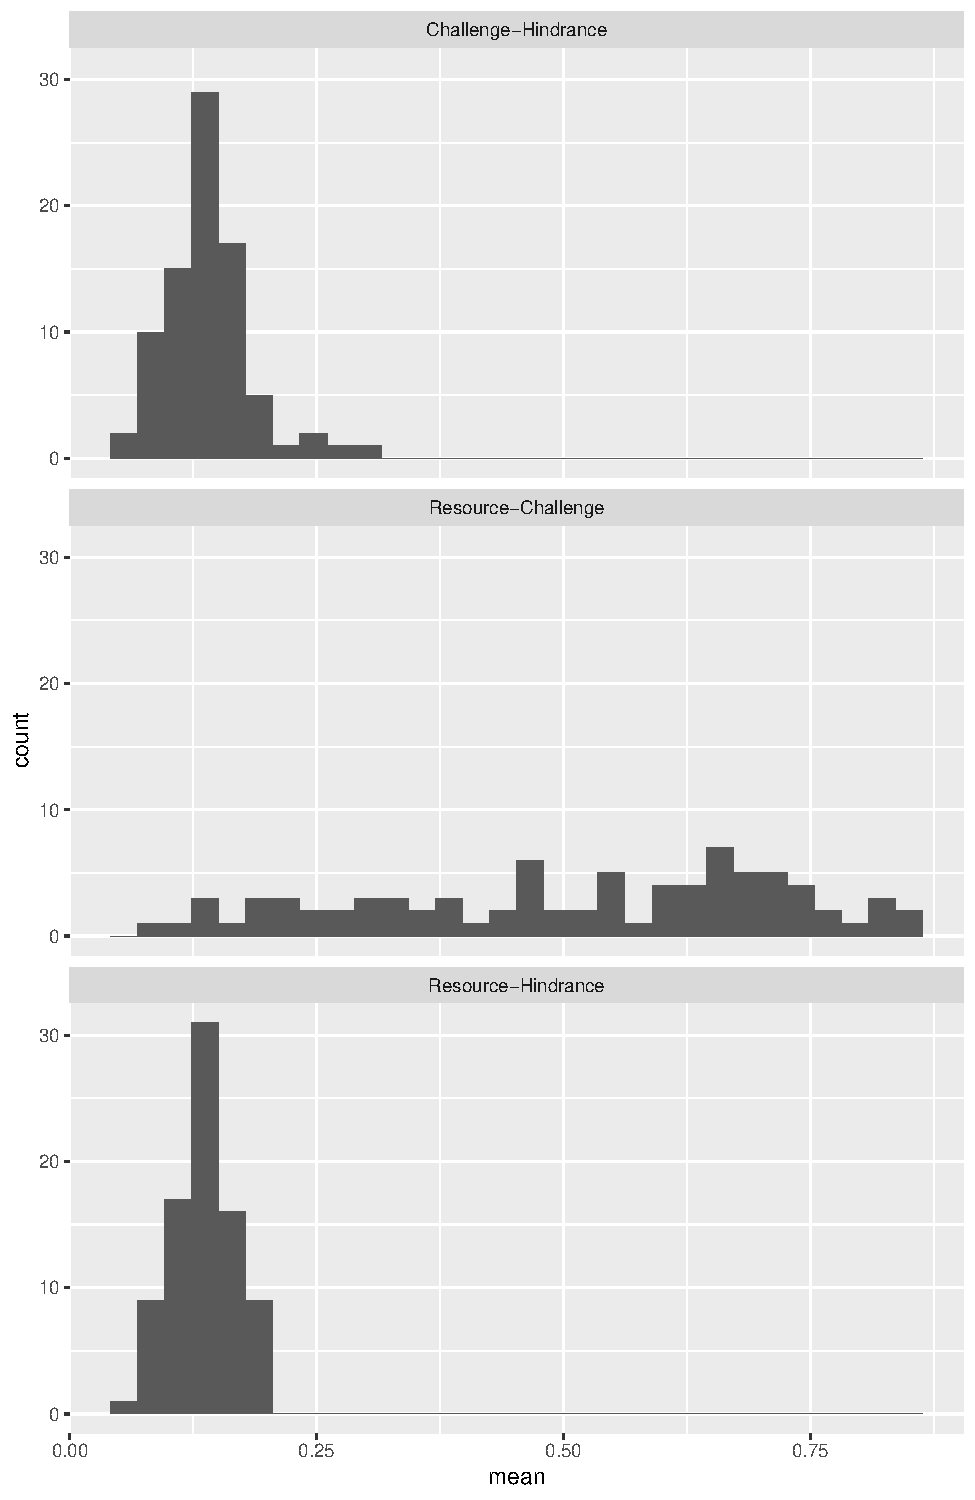
\includegraphics{convergence_files/figure-latex/percagree-1.pdf}
\caption{\label{fig:percagree}Percent convergence (characteristic rated consistently as, for example, both a resource and a hindrance.}
\end{figure}

We next looked for convergence of perception at the level of each individual job characteristic. Here, we calculated the \emph{percent of affirmative correspondence} between individual characteristic perceptions. That is, a respondent needed to agree that \emph{\ldots being in contact with others} was both a resource as well as a challenge in order to be implicated as affirmatively agreeing. We did this for each of the 84 individual characteristics that were rated as a resource, challenge, or demand and then computed an aggregate level of affirmative correspondence for each person. Figure \ref{fig:percagree} presents the results of these correspondences, showing that there was not much mutual agreement regarding characteristics being viewed as both hindrances and resources (\(\bar{X}\) = 0.14) or as challenges and hindrances
(\(\bar{X}\) = 0.14). However, when a characteristic was viewed a resource, it was more likely to also be percieved as a challenge (although the correspondence also exhibited quite a bit of variability; \(\bar{X}\) = 0.51, \emph{sd} = 0.21).

\begin{figure}
\centering
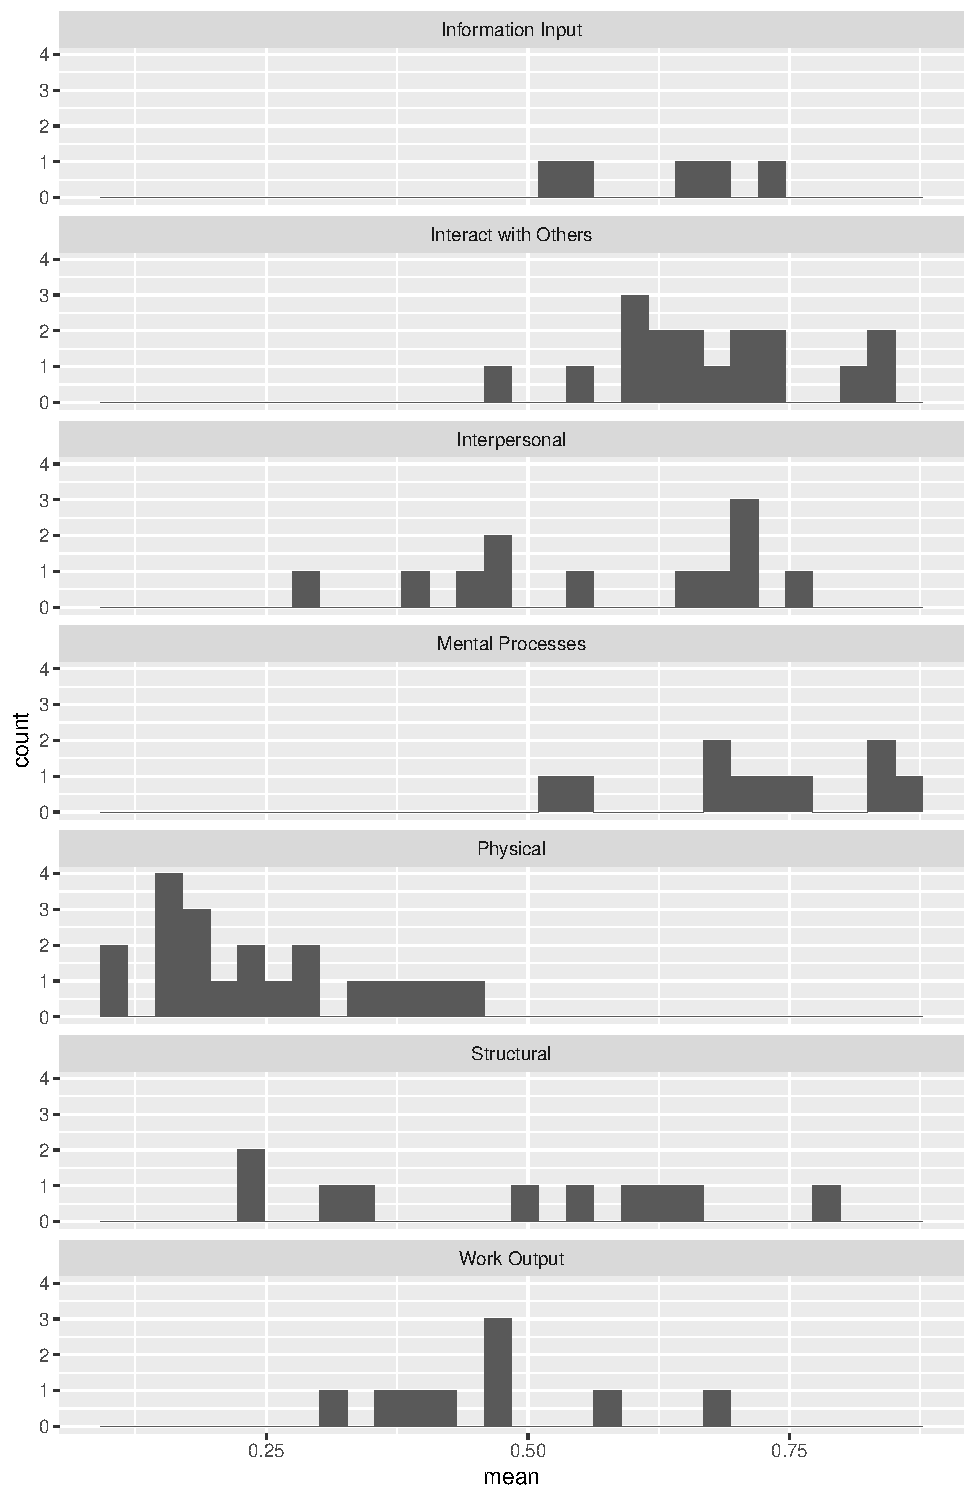
\includegraphics{convergence_files/figure-latex/recchall-1.pdf}
\caption{\label{fig:recchall}Resource and challenge agreement across ONet characteristic groupings (e.g., scales).}
\end{figure}

Figure \ref{fig:recchall} explores the possibility of moderation by \emph{type of characteristic rated} for the resource-challenge convergence. Here we categorized each characteristic by its O*Net ``scale'' (one of seven), and the graph shows greater consistency across certain characteristics (for example, \emph{Mental Processes} or \emph{Interacting with Others}) and less convergence across other \emph{types} of job activities (for example, \emph{Physical} characteristics). A repeated-measures ANOVA retaining these 7 scales as independent variables yielded a treatment effect of \(F_(6, 3,402)\) = 613.5, \emph{p} \textless{} .001 (the subjects' effect was \(F_{(567, 3402)}\) = 6.13, \emph{p} \textless{} .001.

\hypertarget{discussion}{%
\section{Discussion}\label{discussion}}

Our findings highlight the importance of dissociating the \emph{nature} of job demands. Similar to the eustress/distress distinction (e.g., Selye, 1974), it would seem as though demands should be thought of in a valenced manner (e.g., is it a ``good'' demand or a ``bad'' demand)\footnote{Beyond this SIOP presentation, we have further investigated differential associations of challenges and hindrances with ``good'' and ``bad'' outcomes, but have not confirmed meaningful differential associations within this current dataset.}.

The major goal of this paper was to further explore the relationships among total perceived challenge demands, hindrance demands, and resources and outcomes of engagement, stress, and burnout. Additionally, we considered whether resources and challenge demands were perceived as distinct, and finally, whether the patterns were similar across job categories/types of work. The results suggest a positive relationship between both resources and engagement (H1a), and challenge demands and engagement (H2a). Employers would benefit from understanding that at leas the perception of having ``more'' resources and more challenge demands in a job is highly associated with reported engagement. While not a causal relationship, it points to the potential value of these kinds of employee support nonetheless. The other relationships with outcomes of stress and burnout were not supported, suggesting that the sheer number of resources, challenges, and hindrances are not significantly related to these negative outcomes. It is possible that rather than volume, categorically some demands are more related to these outcomes than others.
Further, total resources were highly associated challenge demands (supporting H4). We could even argue, given the magnitude of the correlation, that they are capturing the same thing (74\% overlap with a correlation of .86). Need to also talk about our exploratory findings regarding patterns across job type

\hypertarget{limitations-and-future-directions}{%
\subsection{Limitations and Future Directions}\label{limitations-and-future-directions}}

As with any piece of research, the process and results have limitations, but also provide a variety of additional directions to pursue in the future. First, while a strength of this project, arguably, is the use of O\emph{Net items, practical considerations limited the number of job characteristics we could include in our survey. Future study could consider additional or other O}Net items. We conceptualized resources and demands in terms of perceived total amounts. It may be the case that certain kinds of resources or challenges are more strongly associated with engagement than others, and such, future research could explore the importance of resources/challenges categorically. Further, our study was limited to three outcomes of interest. It would be especially interesting to explore additional outcomes (e.g., job satisfaction) as well, or whether volume of resources and demands operationalized in this way are related to other behaviors (e.g., turnover intention, perceived organizational support, commitment).

\hypertarget{references}{%
\section*{References}\label{references}}
\addcontentsline{toc}{section}{References}

\hypertarget{refs}{}
\begin{CSLReferences}{1}{0}
\leavevmode\hypertarget{ref-abbas2019challenge}{}%
Abbas, M., \& Raja, U. (2019). Challenge-hindrance stressors and job outcomes: The moderating role of conscientiousness. \emph{Journal of Business and Psychology}, \emph{34}(2), 189--201.

\leavevmode\hypertarget{ref-bakker2014job}{}%
Bakker, A. B., \& Demerouti, E. (2014). Job demands--resources theory. \emph{Wellbeing: A Complete Reference Guide}, 1--28.

\leavevmode\hypertarget{ref-bakker2017job}{}%
Bakker, A. B., \& Demerouti, E. (2017). Job demands--resources theory: Taking stock and looking forward. \emph{Journal of Occupational Health Psychology}, \emph{22}(3), 273.

\leavevmode\hypertarget{ref-bakker2007job}{}%
Bakker, A. B., Hakanen, J. J., Demerouti, E., \& Xanthopoulou, D. (2007). Job resources boost work engagement, particularly when job demands are high. \emph{Journal of Educational Psychology}, \emph{99}(2), 274.

\leavevmode\hypertarget{ref-bakker2013weekly}{}%
Bakker, A. B., \& Sanz-Vergel, A. I. (2013). Weekly work engagement and flourishing: The role of hindrance and challenge job demands. \emph{Journal of Vocational Behavior}, \emph{83}(3), 397--409.

\leavevmode\hypertarget{ref-bakker2003dual}{}%
Bakker, A., Demerouti, E., \& Schaufeli, W. (2003). Dual processes at work in a call centre: An application of the job demands--resources model. \emph{European Journal of Work and Organizational Psychology}, \emph{12}(4), 393--417.

\leavevmode\hypertarget{ref-cavanaugh2000empirical}{}%
Cavanaugh, M. A., Boswell, W. R., Roehling, M. V., \& Boudreau, J. W. (2000). An empirical examination of self-reported work stress among US managers. \emph{Journal of Applied Psychology}, \emph{85}(1), 65.

\leavevmode\hypertarget{ref-crawford2010linking}{}%
Crawford, E. R., LePine, J. A., \& Rich, B. L. (2010). Linking job demands and resources to employee engagement and burnout: A theoretical extension and meta-analytic test. \emph{Journal of Applied Psychology}, \emph{95}(5), 834.

\leavevmode\hypertarget{ref-demerouti2001job}{}%
Demerouti, E., Bakker, A. B., Nachreiner, F., \& Schaufeli, W. B. (2001). The job demands-resources model of burnout. \emph{Journal of Applied Psychology}, \emph{86}(3), 499.

\leavevmode\hypertarget{ref-gerich2017relevance}{}%
Gerich, J. (2017). The relevance of challenge and hindrance appraisals of working conditions for employees' health. \emph{International Journal of Stress Management}, \emph{24}(3), 270.

\leavevmode\hypertarget{ref-lazarus1984stress}{}%
Lazarus, R. S., \& Folkman, S. (1984). \emph{Stress, appraisal, and coping}. Springer publishing company.

\leavevmode\hypertarget{ref-podsakoff2007differential}{}%
Podsakoff, N. P., LePine, J. A., \& LePine, M. A. (2007). Differential challenge stressor-hindrance stressor relationships with job attitudes, turnover intentions, turnover, and withdrawal behavior: A meta-analysis. \emph{Journal of Applied Psychology}, \emph{92}(2), 438.

\leavevmode\hypertarget{ref-searle2015merits}{}%
Searle, B. J., \& Auton, J. C. (2015). The merits of measuring challenge and hindrance appraisals. \emph{Anxiety, Stress, \& Coping}, \emph{28}(2), 121--143.

\leavevmode\hypertarget{ref-selye1936syndrome}{}%
Selye, H. (1936). A syndrome produced by diverse nocuous agents. \emph{Nature}, \emph{138}(3479), 32--32.

\leavevmode\hypertarget{ref-selye1974stress}{}%
Selye, H. (1974). \emph{Stress without distress}. Lippincott Williams \& Wilkins.

\leavevmode\hypertarget{ref-webster2011extending}{}%
Webster, J. R., Beehr, T. A., \& Love, K. (2011). Extending the challenge-hindrance model of occupational stress: The role of appraisal. \emph{Journal of Vocational Behavior}, \emph{79}(2), 505--516.

\end{CSLReferences}


\end{document}
